\documentclass[english,,man]{apa6}
\usepackage{lmodern}
\usepackage{amssymb,amsmath}
\usepackage{ifxetex,ifluatex}
\usepackage{fixltx2e} % provides \textsubscript
\ifnum 0\ifxetex 1\fi\ifluatex 1\fi=0 % if pdftex
  \usepackage[T1]{fontenc}
  \usepackage[utf8]{inputenc}
\else % if luatex or xelatex
  \ifxetex
    \usepackage{mathspec}
  \else
    \usepackage{fontspec}
  \fi
  \defaultfontfeatures{Ligatures=TeX,Scale=MatchLowercase}
\fi
% use upquote if available, for straight quotes in verbatim environments
\IfFileExists{upquote.sty}{\usepackage{upquote}}{}
% use microtype if available
\IfFileExists{microtype.sty}{%
\usepackage{microtype}
\UseMicrotypeSet[protrusion]{basicmath} % disable protrusion for tt fonts
}{}
\usepackage{hyperref}
\hypersetup{unicode=true,
            pdftitle={Continuous developmental change explains discontinuities in word learning},
            pdfauthor={Abdellah Fourtassi, Sophie Regan, \& Michael C. Frank},
            pdfkeywords={word learning, cognitive development, computational modeling},
            pdfborder={0 0 0},
            breaklinks=true}
\urlstyle{same}  % don't use monospace font for urls
\ifnum 0\ifxetex 1\fi\ifluatex 1\fi=0 % if pdftex
  \usepackage[shorthands=off,main=english]{babel}
\else
  \usepackage{polyglossia}
  \setmainlanguage[]{english}
\fi
\usepackage{graphicx,grffile}
\makeatletter
\def\maxwidth{\ifdim\Gin@nat@width>\linewidth\linewidth\else\Gin@nat@width\fi}
\def\maxheight{\ifdim\Gin@nat@height>\textheight\textheight\else\Gin@nat@height\fi}
\makeatother
% Scale images if necessary, so that they will not overflow the page
% margins by default, and it is still possible to overwrite the defaults
% using explicit options in \includegraphics[width, height, ...]{}
\setkeys{Gin}{width=\maxwidth,height=\maxheight,keepaspectratio}
\IfFileExists{parskip.sty}{%
\usepackage{parskip}
}{% else
\setlength{\parindent}{0pt}
\setlength{\parskip}{6pt plus 2pt minus 1pt}
}
\setlength{\emergencystretch}{3em}  % prevent overfull lines
\providecommand{\tightlist}{%
  \setlength{\itemsep}{0pt}\setlength{\parskip}{0pt}}
\setcounter{secnumdepth}{0}
% Redefines (sub)paragraphs to behave more like sections
\ifx\paragraph\undefined\else
\let\oldparagraph\paragraph
\renewcommand{\paragraph}[1]{\oldparagraph{#1}\mbox{}}
\fi
\ifx\subparagraph\undefined\else
\let\oldsubparagraph\subparagraph
\renewcommand{\subparagraph}[1]{\oldsubparagraph{#1}\mbox{}}
\fi

%%% Use protect on footnotes to avoid problems with footnotes in titles
\let\rmarkdownfootnote\footnote%
\def\footnote{\protect\rmarkdownfootnote}


  \title{Continuous developmental change explains discontinuities in word
learning}
    \author{Abdellah Fourtassi\textsuperscript{1}, Sophie Regan\textsuperscript{1},
\& Michael C. Frank\textsuperscript{1}}
    \date{}
  
\shorttitle{Continuous Development of Word Learning}
\affiliation{
\vspace{0.5cm}
\textsuperscript{1} Department of Psychology, Stanford University}
\keywords{word learning, cognitive development, computational modeling}
\usepackage{csquotes}
\usepackage{upgreek}
\captionsetup{font=singlespacing,justification=justified}

\usepackage{longtable}
\usepackage{lscape}
\usepackage{multirow}
\usepackage{tabularx}
\usepackage[flushleft]{threeparttable}
\usepackage{threeparttablex}

\newenvironment{lltable}{\begin{landscape}\begin{center}\begin{ThreePartTable}}{\end{ThreePartTable}\end{center}\end{landscape}}

\makeatletter
\newcommand\LastLTentrywidth{1em}
\newlength\longtablewidth
\setlength{\longtablewidth}{1in}
\newcommand{\getlongtablewidth}{\begingroup \ifcsname LT@\roman{LT@tables}\endcsname \global\longtablewidth=0pt \renewcommand{\LT@entry}[2]{\global\advance\longtablewidth by ##2\relax\gdef\LastLTentrywidth{##2}}\@nameuse{LT@\roman{LT@tables}} \fi \endgroup}


\DeclareDelayedFloatFlavor{ThreePartTable}{table}
\DeclareDelayedFloatFlavor{lltable}{table}
\DeclareDelayedFloatFlavor*{longtable}{table}
\makeatletter
\renewcommand{\efloat@iwrite}[1]{\immediate\expandafter\protected@write\csname efloat@post#1\endcsname{}}
\makeatother
\usepackage{lineno}

\linenumbers
\usepackage[titles]{tocloft}
\cftpagenumbersoff{figure}
\renewcommand{\cftfigpresnum}{\itshape\figurename\enspace}
\renewcommand{\cftfigaftersnum}{.\space}
\setlength{\cftfigindent}{0pt}
\setlength{\cftafterloftitleskip}{0pt}
\settowidth{\cftfignumwidth}{Figure 10.\qquad}
\usepackage{tipa}
\usepackage[sortcites=false,sorting=none]{biblatex}

\authornote{

None of the authors have any financial interest or a conflict of
interest regarding this work and this submission.

Correspondence concerning this article should be addressed to Abdellah
Fourtassi, Postal address. E-mail:
\href{mailto:afourtas@stanford.edu}{\nolinkurl{afourtas@stanford.edu}}}

\abstract{
``Cognitive development is often characterized in terms of
discontinuities, but these discontinuities can sometimes be apparent
rather than actual and can arise from continuous developmental change.
To explore this idea, we use as a case study the finding by Stager and
Werker (1997) that children's early ability to distinguish similar
sounds does not automatically translate into word learning skills. Early
explanations proposed that children may not be able to encode subtle
phonetic contrasts when learning novel word meanings, thus suggesting a
discontinuous/stage-like pattern of development. However, later work has
revealed (e.g., through using more precise testing methods) that
children do encode such contrasts, thus favoring a continuous pattern of
development. Here we propose a probabilistic model that represents word
knowledge in a graded fashion and characterizes developmental change as
improvement in the precision of this graded knowledge. Our model
explained previous findings in the literature and provided a new
prediction --- the referents' visual similarity modulates word learning
accuracy. The models' predictions were corroborated by human data we
collected from both preschool children and adults. The broader impact of
this work is to show that computational models, such as ours, can help
us explore the extent to which episodes of cognitive development that
are typically thought of as discontinuities may emerge from simpler,
continuous mechanisms.''


}

\usepackage{amsthm}
\newtheorem{theorem}{Theorem}[section]
\newtheorem{lemma}{Lemma}[section]
\theoremstyle{definition}
\newtheorem{definition}{Definition}[section]
\newtheorem{corollary}{Corollary}[section]
\newtheorem{proposition}{Proposition}[section]
\theoremstyle{definition}
\newtheorem{example}{Example}[section]
\theoremstyle{definition}
\newtheorem{exercise}{Exercise}[section]
\theoremstyle{remark}
\newtheorem*{remark}{Remark}
\newtheorem*{solution}{Solution}
\begin{document}
\maketitle

\section{Introduction}\label{introduction}

Cognitive development is often characterized in terms of a succession of
discontinuous stages. In Piaget's initial conception, these stages
cross-cut different aspects of cognition (Piaget, 1954); in more modern
conceptions, distinct domains are often thought to progress on their own
timeline (e.g., Carey, Zaitchik, \& Bascandziev, 2015). Although
intuitively appealing, this sort of stage theory can be challenging to
integrate with theories of learning, which typically posit that
knowledge and skills improve incrementally with experience. Indeed, one
of the central challenges of cognitive development has been to explain
transitions between stages which appear to be qualitatively different
(Carey, 2009).

Nevertheless, at least in some cases, development may only appear to be
stage-like. Some discontinuities may be related to how we measure a
specific skill. Other discontinuities may emerge due to statistical
thresholding (e.g., an experimental p-value of \(p < .05\) for one age
group but not another) which can create a spurious dichotomy between
success and failure in observing a given behavior. In such cases,
positing discontinuous stages is unnecessary. Instead, a continuous
model --- involving similar representations across the lifespan --- may
provide a simpler and more transparent account of development (cf.
McMurray, 2007; Shultz, Schmidt, Buckingham, \& Mareschal, 1995).

To explore this point computationally, we use a case study from word
learning literature. Stager and Werker (1997) first showed that
children's early ability to distinguish similar sounds does not
automatically translate into word learning skills. The authors measured
word learning using an audio-visual habituation Switch task. First,
infants are familiarized with two word-object pairings (e.g., label 1
with object 1 and label 2 with object 2). Second, they are tested using
two types of trials. The control \enquote{same} trial consists of a
correct pairing (e.g., label 1 with object 1) and the \enquote{switch}
trial consists of a wrong pairing (e.g., label 1 with object 2). If
babies have correctly learned the association during the habituation,
they are supposed to be surprised by the \enquote{switch} trial and not
by the \enquote{same} trial. The former should thus result in a greater
looking time compared to the latter (Werker, Cohen, Lloyd, Casasola, \&
Stager, 1998).

Though infants around 14-month old can distinguish perceptually similar
sound pairs such as \enquote{dih} and \enquote{bih}, they appear to fail
in mapping this pair to two different objects in the switch task. This
failure was initially taken as evidence that 14-month olds do not encode
subtle sounds during meaning learning (Pater, Stager, \& Werker, 2004;
Stager \& Werker, 1997). This interpretation suggested a
discontinuous/stage-like pattern of development whereby younger children
fail to encode the contrastive phonetic detail, whereas older children,
around 17 months, typically do (Werker, Fennell, Corcoran, \& Stager,
2002).

The initial discontinuous interpretation has been challenged by
subsequent work. For instance, Yoshida, Fennell, Swingley, and Werker
(2009) investigated whether failure in the Switch task reflects a lack
of sound encoding during \emph{habituation}, or whether it is only due
to the nature of the \emph{testing} method which does not allow learning
below a certain threshold to be detected. They used the same habituation
procedure as Stager and Werker (1997), but instead of comparing the
looking times in \enquote{same} and \enquote{switch} trials, they tested
infants using a two-alternative choice task comparing fixations to
target and distractor objects (Fernald, Perfors, \& Marchman, 2006;
Golinkoff, Hirsh-Pasek, Cauley, \& Gordon, 1987). Using this testing
method, researchers found evidence for learning even in 14-month olds.

Another challenge to the discontinuous account of development came from
adult studies. If the mismatch between sound discrimination and word
learning is only a stage in early infancy, then this mismatch should
disappear by adulthood. Nonetheless, even adults show patterns of
learning that mirror those shown by 14-month-olds when the sound
contrasts are more challenging (Pajak, Creel, \& Levy, 2016; White, Yee,
Blumstein, \& Morgan, 2013).

Some researchers (Pajak et al., 2016; Swingley, 2007; Yoshida et al.,
2009) proposed that word knowledge may not be encoded in a binary
fashion, i.e., it is not the case that children either succeed or fail
in encoding minimal contrast when learning the meanings. Rather, they
may be encoding this knowledge in a graded fashion (see Munakata (2001)
for an detailed discussion of a similar view). Thus, development does
not so much involve a qualitative shift (i.e., a sudden emergence of an
ability that did not exist before) as much as it consists in the
continuous refinement of initially noisy knowledge.

Many different computational formalisms can represent graded knowledge.
Here we use probabilistic models, a formalism that allows both easy
examination of internal representations and quantification of the
robustness of these representations. Word knowledge can be characterized
with a probability distribution over sound instances organized in a
similarity space. The probability is highest at the most typical sound
instance. It decreases as the instance becomes less typical. The
precision of word knowledge can be characterized by whether it tolerates
slightly atypical pronunciations. This tolerance is captured formally by
the variance of the probability distribution: larger variance indicates
higher tolerance and lower precision, whereas smaller variance indicates
lower tolerance and higher precision (for an illustration, see Figure
\ref{fig:illus} top and right panels).

This general framework --- in which the precision of word knowledge is
characterized with the variance of a probability distribution --- can
already provide an intuitive way of thinking about several findings. In
particular, unlike the binary view, the probabilistic view allows for
the possibility of word knowledge being both successful and noisy. This
new understanding can provide an account for the fact that children show
evidence of learning in some testing condition (e.g., Yoshida et al.,
2009) but not in others (e.g., Stager \& Werker, 1997) --- depending on
the precision of the measurement.

In a word-pair learning paradigm, children are supposed to associate one
label, e.g., \enquote{bih}, with object 1 and a second label, e.g.,
\enquote{dih}, with object 2. Infants may succeed in learning both
associations. Nevertheless, the variance with which the pair of words
are encoded can still be large, causing their probability distributions
to overlap (Figure \ref{fig:illus}, top). The way this (noisy) knowledge
is probed can lead to different results.

In the Switch task (Stager \& Werker, 1997), children are understood to
succeed if they reject a wrong association (e.g., \enquote{bih} with
object 2). However, a large overlap between \enquote{bih} and
\enquote{dih} means that \enquote{bih} is itself a plausible
mispronunciation of \enquote{dih}. The wrong association may not be
rejected by children because the speaker could have said \enquote{bih}
but meant \enquote{dih}. In the two-alternative choice task (Yoshida et
al., 2009), children do not have to reject the wrong association; they
only need to show a preference, albeit small, for the correct one. Thus,
unlike the Switch, this testing method allows us to see subtle evidence
of learning even with a large overlap. For example, given the label
\enquote{bih}, children are supposed to pick which object is a better
match to this label. Though it is possible that the speaker said
\enquote{bih} and meant \enquote{dih}, it is \emph{more} likely that the
speaker both said and meant \enquote{bih} --- this higher probability
leads to a preference for the correct object.

In addition to explaining the difference in behavior across the Switch
and the preferential looking tasks, the probabilistic account explains
difference in behavior within the same task. In particular, when the
labels are quite distinct in the perceptual space (\enquote{lif} vs.
\enquote{neem}), the probabilistic distributions do not overlap as much
as in the case of similar-sounding words (Figure \ref{fig:illus}, left).
This fact means that the learners will have less tolerance for the wrong
association, leading to a successful rejection in the Switch task (as
was reported by Stager and Werker (1997) and subsequent studies using
the same paradigm). Further, distinctiveness can be enhanced even for
minimally different sounds when other cues highlight their difference
(Dautriche, Swingley, \& Christophe, 2015; Rost \& McMurray, 2009, 2010;
Thiessen, 2007; Yeung \& Werker, 2009).

In this framework, developmental change can be understood as an increase
in the precision (i.e., a decrease in the variance) of the probabilistic
knowledge, leading to a lower overlap between the distributions of
similar-sounding words (Figure \ref{fig:illus}, right). Importantly, a
more precise representation still has a non-zero variance. Thus,
learning difficulties can still be induced with challenging stimuli or
in cognitively demanding situations as was demonstrated in adults
studies (Pajak et al., 2016; White et al., 2013).

\subsection{The current study}\label{the-current-study}

The probabilistic account has been put forward to explain patterns of
learning and development at the qualitative level. However, it is
crucial to have a precise computational instantiation of this account
which would help us 1) test this theoretical hypothesis more directly
and 2) identify the particular parameters that are the locus of
developmental change. One previous study attempted to provide such a
computational instantiation (Hofer \& Levy, 2017). However, this
previous work was designed with the goal of reproducing the results of a
specific study (Pajak et al., 2016) which focused on explaining the
mismatch between speech perception and word learning in adults rather
than on exploring the mechanism of development.

The present work proposes a model of word-pair learning based on the
probabilistic account. We tested the ability of this model to both
\emph{explain} various findings in previous experiments in both children
and adults (e.g., the fact that similar words are harder to learn than
different words) and to \emph{predict} new learning patterns that have
not been tested before. In particular, we test the prediction that
referent similarity (i.e., the confusability of pictures referred to by
novel words) should play an identical computational role to word form
similarity in predicting recognition difficulty. Although this
prediction is intuitive, to our knowledge, it has never been tested.
Finally, we explore the extent to which the probabilistic account allows
us to understand development in terms of as a continuous refinement in
similar representations across the lifespan.

The paper is organized as follows. First, we introduce the model and we
explain how it allows us to characterize behavior in a
word-pair-learning paradigm. Then we explore the predictions of the
model through simulating its behavior across different parameter
settings. Next, we quantify the extent to which the model's predictions
account for human data we collected from both preschool children and
adults. Finally, we discuss the results in the light of existing
accounts of word development.

\begin{figure}

{\centering 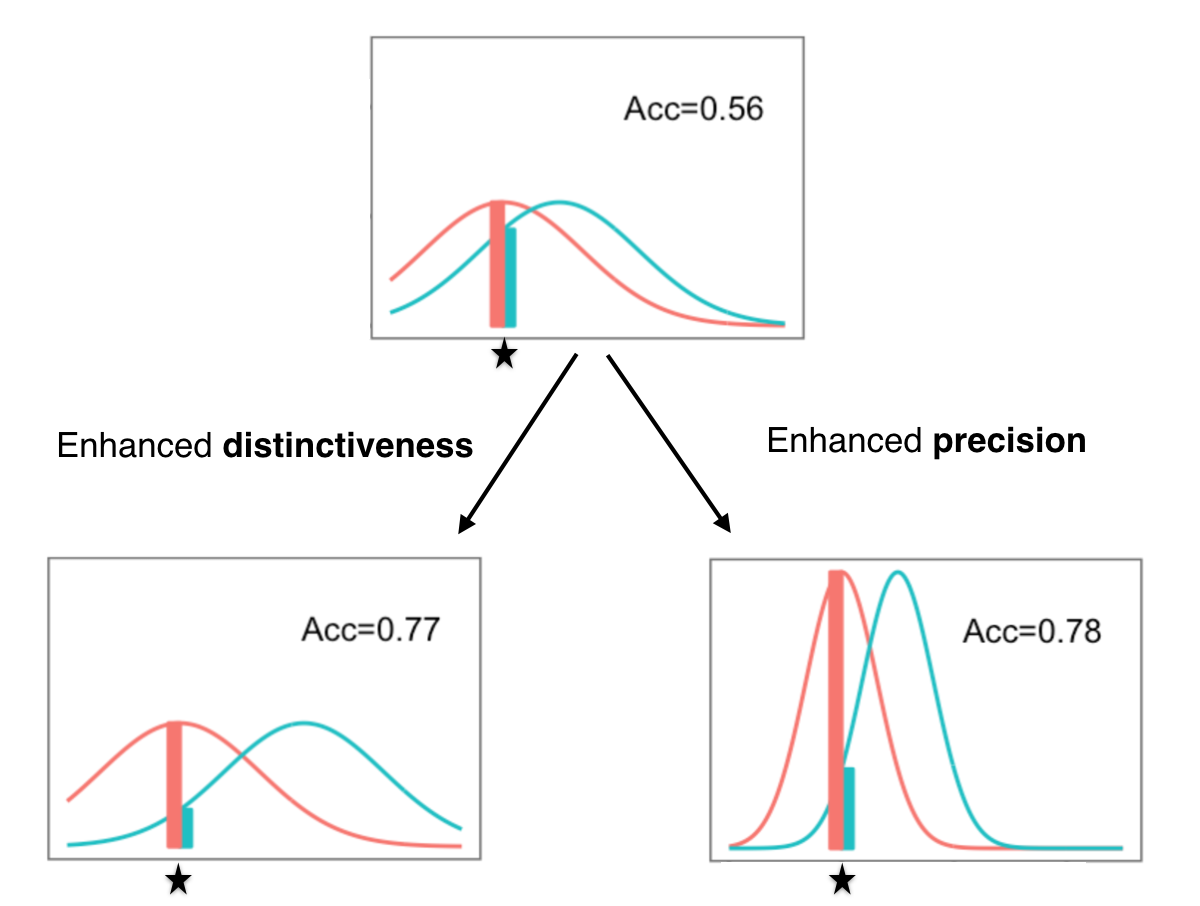
\includegraphics[width=300px]{figs/illustration} 

}

\caption{An illustration of the probabilistic/continuous account using simulated data. A word is represented with a distribution over the perceptual space (indicated in red or blue). When the uncertainty of the representation is large relative to the distance between the stimuli (top panel), an instance of the red category (indicated with a star) could also be a plausible instance of the green category, hence the low recognition accuracy score. The accuracy is higher when the stimuli are less similar (left panel), or when the representation are more precise (right panel).}\label{fig:illus}
\end{figure}

\section{Model}\label{model}

\subsection{Probabilistic structure}\label{probabilistic-structure}

Our model consists of a set of variables describing the general process
of spoken word recognition in a referential situation. These variables
are related in a way that reflects the simple generative scenario
represented graphically in Figure \ref{fig:model}. When a speaker utters
a sound in the presence of an object, the observer assumes that the
object \(o\) activated the concept \(C\) in the speaker's mind. The
concept prompted the corresponding label \(L\). Finally, the label was
physically instantiated by the sound \(s\).

\begin{figure}

{\centering 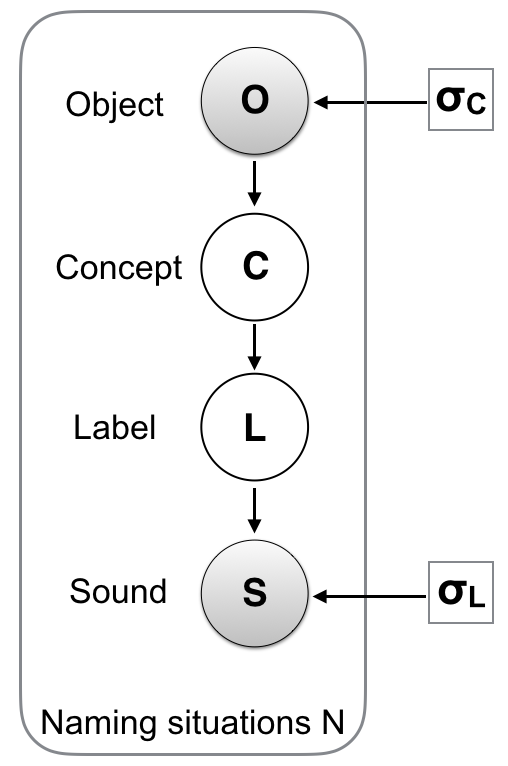
\includegraphics[width=150px]{figs/model} 

}

\caption{Graphical representation of our model. Circles indicate random variables (shading indicates observed variables). The squares indicate fixed model parameters.}\label{fig:model}
\end{figure}

A similar probabilistic structure was used by Lewis and Frank (2013) to
model concept learning, and by Hofer and Levy (2017) to model spoken
word learning. However, the first study assumed that the sounds are
heard unambiguously, and the second assumed the concepts are observed
unambiguously. In our model, we assume that both labels and concepts are
observed with a certain amount of perceptual noise, which we assume, for
simplicity, is captured by a normal distribution:

\begin{equation} \label{eq:object}
 p(o | C) \sim  \mathcal{N}(\mu_C, \sigma^2_C) 
\end{equation}

\begin{center}
and 
\end{center}

\begin{equation} \label{eq:sound}
p(s| L) \sim  \mathcal{N}(\mu_L, \sigma^2_L)
\end{equation}

Finally, we assume there to be one-to-one mappings between concepts and
labels and that observers have successfully learned these mappings
during the exposure phase:

\begin{equation}
P(L_i|C_j) = 
\begin{cases}
  1 & \text{if  }  i=j \\  
  0  & \text{otherwise  }
\end{cases}
\end{equation}

\subsection{Inference}\label{inference}

In our canonical inference case, the learner hears a sound \(s\) and has
to decide which object \(o\) provides an optimal match to this sound
(see Figure \ref{fig:task}). To this end, they must compute the
probability \(P(o|s)\) for all possible objects. This probability can be
computed by summing over all possible concepts and labels:

\begin{equation}
P(o|s)=\sum_{C,L} P(o, C, L| s)  
\end{equation}

Using the fact that \(P(o,C,L|s) = \frac{P(o,C,L,s)}{P(s)}\) and that
\(P(s)\) does not depend on \(o\), we arrive at the equation:

\begin{equation}
P(o|s) \propto \sum_{C,L} P(o, C, L, s) 
\end{equation}

The joint probability \(P(o,C,L,s)\) is obtained by factoring the
graphical model in Figure \ref{fig:model}:

\[P(o,C,L,s) = P(s|L)P(L|C)P(C|o)P(o)\]

Using Bayes' rule, we can rewrite \(P(C|o)\) in terms of \(P(o|C)\):

\[P(C|o) = \frac{P(o|C)P(C)}{P(o)}\]

By subtituting this term in the expression of the joint distribution
\(P(o,C,L,S)\) we obtain:

\[P(o,C,L,s) = P(s|L)P(L|C)P(o|C)P(C)\]

Finally, assuming that the concepts' prior probability \(P(C)\) is
uniformly
distributed,\footnote{This is a reasonable assumption in our particular case given the similarity of the concept pairs used in each naming situation in our experiment.}
we obtain the following expression, where all conditional dependencies
are now well defined:

\begin{equation} \label{eq:general}
P(o|s) \propto \sum_{C,L}  P(s|L)P(L|C)P(o|C)
\end{equation}

\subsection{Task and model
predictions}\label{task-and-model-predictions}

\begin{figure}[t]

{\centering 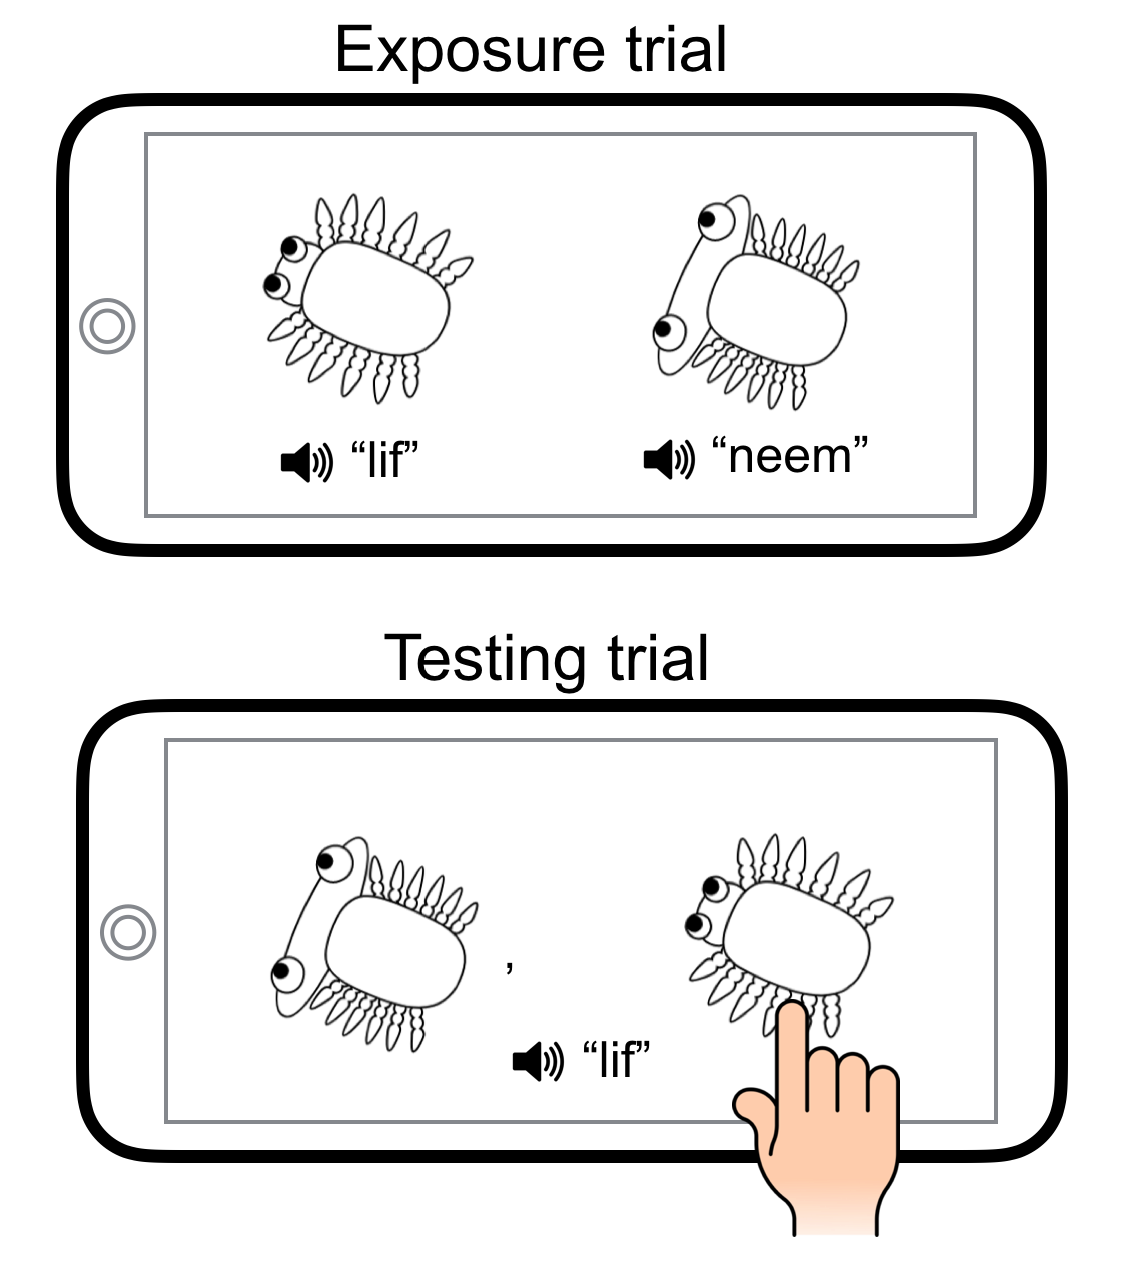
\includegraphics[width=3.75in]{figs/task} 

}

\caption{An overview of the task used in this study.}\label{fig:task}
\end{figure}

We use the model to predict word learning in a task similar to the one
introduced by Stager and Werker (1997). We used a modified version of
the task where the testing method consists in a two-alternative
forced-choice (Yoshida et al., 2009). In this task, participants are
first exposed to two different word-object pairings (e.g., \enquote{lif}
- object 1, \enquote{neem} - object 2). The word-object associations are
introduced sequentially. After this exposure phase, participants perform
a series of test trials. In each of these trials, one of the two sounds
is uttered (e.g., \enquote{lif}) and participants choose the
corresponding object from the two alternatives. An overview of the task
is shown in Figure \ref{fig:task}.

\subsubsection{Model 1}\label{model-1}

From the general expression \ref{eq:general}, we derive three exact
analytical solutions instantiating different learning assumptions.
Recall from expressions \ref{eq:object} and \ref{eq:sound} that
\(P(o|C)\) and \(P(s|L)\) have parameters \(\sigma_C\) and \(\sigma_L\),
respectively, that control perceptual uncertainty. The first solution is
derived by assuming that the labels are recovered from sounds with a
certain level of uncertainty \(\sigma_L > 0\), but that concepts are
unambiguously recovered from the observed objects, i.e.,
\(\sigma_C \rightarrow 0\). This assumption has been made --- whether
implicitly or explicitly --- by most previous work in this line of
research. For example, in Stager and Werker (1997), the objects were
quite dissimilar. Thus, the assumption that they were easily
discriminated by infants seems relatively well justified. One important
implication of this assumption is that only the similarity of word
sounds modulates success in word learning, not the similarity of the
referents (as long as these referents are differentiated perceptually).
This assumption yields the following probability function:

\begin{equation} \label{eq:model1}
P(o_T|s)= \frac{1}{1 + e^{-\frac{\Delta s^2}{2\sigma_L^2}}}
\end{equation}

where \(\Delta s = s_2-s_1\).

\subsubsection{Model 2}\label{model-2}

The second solution is derived by making the more general assumption
that both the labels and the concepts are recovered with noise from the
sounds and objects. We first introduce the simplifying assumption that
the label-related uncertainty \(\sigma_L\) and the concept-related
uncertainty \(\sigma_C\) are of a similar magnitude, i.e.,
\(\sigma_C \approx \sigma_L = \sigma\). This assumption makes the
prediction that the sound similarity and the object similarity impact
word learning accuracy in exactly the same way. Furthermore, it allows
us to study the behavior of the model with only one free parameter, an
important consideration given the small number of datapoints available
from any given infant experiment.

\begin{equation} \label{eq:model2}
P(o_T|s)= \frac{1 + e^{- \frac{\Delta s^2 + \Delta o^2}{2\sigma^2}}}{1 + e^{-\frac{\Delta s^2 + \Delta o^2}{2\sigma^2}}+ e^{-\frac{\Delta s^2}{2\sigma^2}} + e^{-\frac{\Delta o^2}{2\sigma^2}}}
\end{equation}

\subsubsection{Model 3}\label{model-3}

We finally derive the third (and most general) solution which allows
label- and concept-related uncertainties to vary independently.

\begin{equation} \label{eq:model3}
P(o_T|s)= \frac{1 + e^{- (\frac{\Delta s^2}{2\sigma_L^2}+ \frac{\Delta o^2}{2\sigma_C^2})}}{1 + e^{-(\frac{\Delta s^2}{2\sigma_L^2}+ \frac{\Delta o^2}{2\sigma_C^2})}+ e^{-\frac{\Delta s^2}{2\sigma_L^2}} + e^{-\frac{\Delta o^2}{2\sigma_C^2}}}
\end{equation}

In order to understand the predictions of the models (especially the
more general ones, i.e., Model 2 and 3), Figure \ref{fig:simulation}
show simulations of the accuracy \(P(o_T|s)\) as a function of the
distinctiveness parameters (\(\Delta s\) and \(\Delta o\)) and the
uncertainty parameters \(\sigma_L\) and \(\sigma_C\).

\begin{figure}[htbp]
\centering
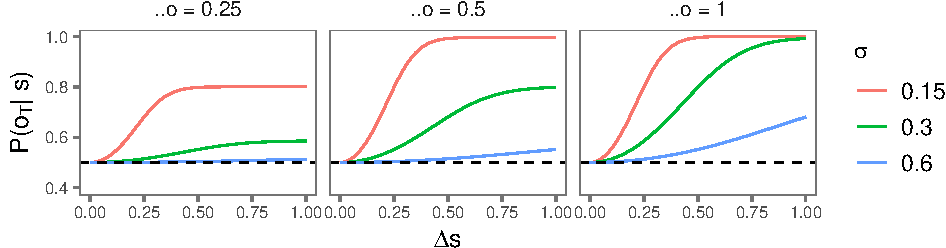
\includegraphics{ms_blind_files/figure-latex/simulation-1.pdf}
\caption{\label{fig:simulation}The predicted probability of accurate
responses in the testing phase as a function of stimuli distinctiveness
\(\Delta s\) and \(\Delta o\) and representation precision \(\sigma\)
(For simplicity, we use model 2, which assumes that
\(\sigma\)=\(\sigma_C\)=\(\sigma_L\)). Dashed line represents chance.}
\end{figure}

The simulations explain two experimental results from previous studies
and make one new prediction:

\begin{enumerate}
\def\labelenumi{\arabic{enumi})}
\item
  For fixed values of \(\Delta o\) and \(\sigma\), the probability of
  accurate responses increases as a function of \(\Delta s\). This
  pattern accounts for the fact that similar sounds are generally more
  challenging to learn than different sounds for both children (Stager
  \& Werker, 1997) and adults (Pajak et al., 2016).
\item
  For fixed values of \(\Delta s\) and \(\Delta o\), accuracy increases
  when the representational uncertainty \(\sigma\) decreases. This
  observation provides a simple model for developmental change. Younger
  children have noisier representations (see Swingley, 2007; Yoshida et
  al., 2009), which leads to lower word recognition accuracy, especially
  for similar-sounding words.
\item
  For fixed values of \(\Delta s\) and \(\sigma\), accuracy increases
  with the visual distance between the semantic referents \(\Delta o\).
  This is a new prediction that our model makes. Previous work studied
  the effect of several bottom-up and top-down properties in
  disambiguating similar sounding words (e.g., Fennell \& Waxman, 2010;
  Rost \& McMurray, 2009; Thiessen, 2007), but to our knowledge, no
  previous study in the literature tested the effect of the visual
  distance between the semantic referents.
\end{enumerate}

\section{Experiment}\label{experiment}

In this experiment, we tested participants in the word learning task
introduced above (Figure \ref{fig:task}). More precisely, we explored
the predictions related to both distinctiveness and precision. Sound
similarity (\(\Delta s\)) and object similarity (\(\Delta o\)) were
varied simultaneously in a within-subject design. Two age groups
(preschool children and adults) were tested on the same task\footnote{This
  four-condition within-subject design is relatively novel for
  preschoolers, but we followed the tablet paradigm (e.g., Frank,
  Sugarman, Horowitz, Lewis, \& Yurovsky, 2016) which allowed us to
  gather a relatively large number of trials from each child.} to
explore whether development can be characterized with the uncertainty
parameters, \(\sigma_C\) and \(\sigma_L\). The experiment, sample size,
exclusion criteria, and the model's main predictions were
pre-registered.\footnote{Due to the double-blind review, the link to the osf repository is only provided in the full version addressed to the editor.}

\subsection{Methods}\label{methods}

\subsubsection{Participants}\label{participants}

We report data from \(N=\) 63 children ages 4-5 years from a nursery
school. An additional \(N=\) 39 children participated but were removed
from analyses (using preregistered exclusion criteria) because they were
not above chance on the catch trials due to the challenging nature of
our procedure (see below). We also report data from \(N=\) 74 adult
participants tested on Amazon Mechanical Turk. An additional \(N=\) 26
were tested but removed from analyses (again, using preregistered
exclusion criteria) because they had low scores on the catch trials or
because they were familiar with the non-English sound stimuli we used in
the adult experiment.

\subsubsection{Stimuli and similarity
rating}\label{stimuli-and-similarity-rating}

The sound stimuli were generated using the MBROLA Speech Synthesizer
(Dutoit, Pagel, Pierret, Bataille, \& Van der Vrecken, 1996). We
generated three kinds of nonsense word pairs which varied in their
degree of perceptual similarity to English speakers: 1) \emph{different}
pairs: \enquote{lif}/\enquote{neem} and \enquote{zem}/\enquote{doof}, 2)
\emph{intermediate} pairs: \enquote{aka}/\enquote{ama} and
\enquote{ada}/\enquote{aba}, and 3) \emph{similar} non-English pairs:
\enquote{ada}/\enquote{a\textipa{d\super h}a} (in hindi) and
\enquote{a\textipa{Q}a}/\enquote{a\textipa{\textcrh}a} (in arabic).

As for the objects, we used the Dynamic Stimuli javascript
library\footnote{https://github.com/erindb/stimuli} which allowed us to
generate objects in four different categories: \enquote{tree,}
\enquote{bird,} \enquote{bug,} and \enquote{fish.} These categories were
described to participants as naturally occurring kinds on an alien
planet. In each category, we generated \emph{different},
\emph{intermediate}, and \emph{similar} pairs by manipulating a
continuous property controlling features of the category's shape (e.g.,
body stretch or head fatness).

In order to validate and quantify our similarity scales, we ran a
separate survey on Amazon Mechanical Turk where we asked \(N=20\) adults
participants to evaluate the similarity of each sound and object pair on
a 7-point scale. Data are shown in Figure \ref{fig:stim} where we scaled
responses within the range {[}0,1{]} for each stimulus group. We used
these data in all models as an empirical measurement of the perceptual
distance between the sound pairs and the object pairs. The use of
empirical measurement allows us to eliminate \(\Delta s\) and
\(\Delta s\) as free parameters (see Frank and Goodman (2012) and Xu and
Tenenbaum (2007) for a similar strategy).

\subsubsection{Design}\label{design}

Each age group saw only two of the three levels of similarity described
in the previous sub-section: \emph{different} vs. \emph{intermediate}
for the preschoolers, and \emph{intermediate} vs. \emph{similar} for
adults. We made this choice in light of pilot studies showing that
adults were at ceiling with \emph{different} sounds/objects, and
children were at chance with the \emph{similar} sounds/objects. That
said, this difference in the level of similarity is accounted for in the
model: We used empirical distance measurement to fill in the appropriate
values of \(\Delta s\) and \(\Delta o\) for each age group.

\begin{figure}[h]

{\centering 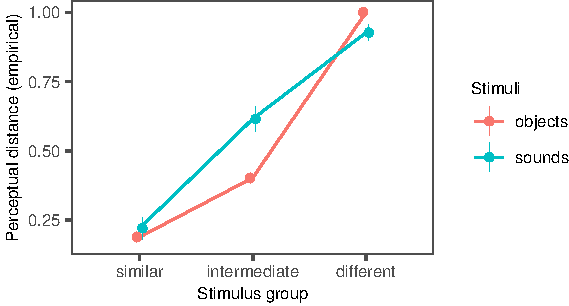
\includegraphics{ms_blind_files/figure-latex/stim-1} 

}

\caption{Distances for both sound and object pairs from an adult norming study. Data represent Likert values normalized to [0,1] interval. Error bars represent 95\% confidence intervals.}\label{fig:stim}
\end{figure}

To maximize our ability to measure subtle stimulus effects, the
experiment was a 2x2 within-subjects factorial design with four
conditions: high/low sound similarity crossed with high/low visual
object similarity. Besides the four conditions, we also tested
participants on a fifth catch condition which was similar in its
structure to the other ones but was trivially easy and used only to
select participants who were able to follow the instructions and show
minimal learning.

\subsubsection{Procedure}\label{procedure}

Preschoolers were tested at the nursery school using a tablet, whereas
adults used their own computers to complete the same experiment online.
Participants were tested in a random sequence of five conditions: the
four experimental conditions plus the catch condition. In each
condition, participants saw a first block of four exposure trials
followed by four testing trials, and a second block of two exposure
trials (for memory refreshment) followed by an additional four testing
trials. The length of this procedure was demanding, especially for
children, but we adopted a fully within-subjects design based on pilot
testing that indicated that precision of measurement was critical for
testing our experimental predictions.

In the exposure trials, participants saw two objects associated with
their corresponding sounds. We presented the first object on the left
side of the tablet's screen simultaneously with the corresponding sound.
The second sound-object association followed on the other side of the
screen after 500ms. For both objects, visual stimuli were present for
the duration of the sound clip (about 800ms). In the testing trials,
participants saw both objects simultaneously and heard only one sound.
They completed the trial by selecting which of the two objects
corresponded to the sound. The object-sound pairings were randomized
across participants, as was the order of the conditions (except for the
catch condition which was always placed in the middle of the testing
sequence). We also randomized the on-screen position (left vs.~right) of
the two pictures on each testing trial.

\begin{figure}[h]

{\centering 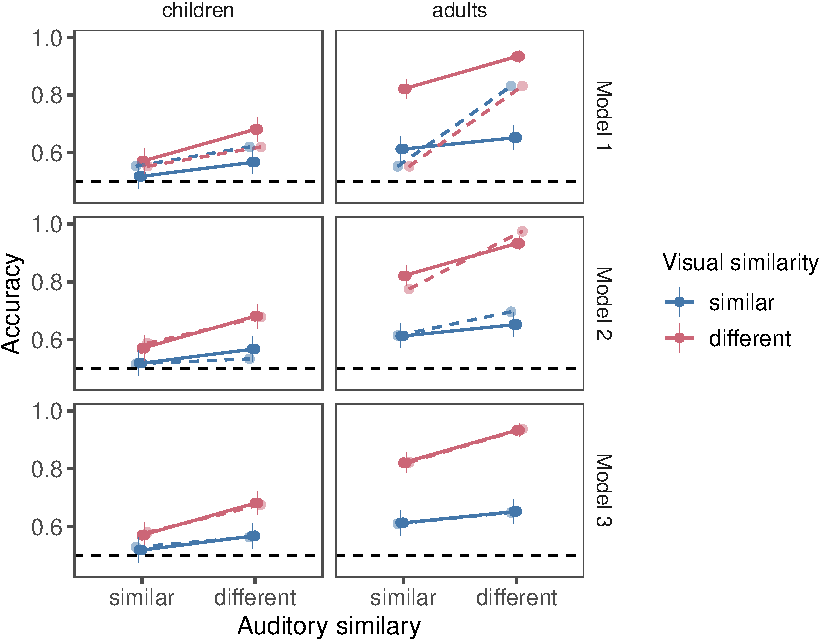
\includegraphics{ms_blind_files/figure-latex/allData-1} 

}

\caption{Accuracy of word recognition as a function of the sound distance, the object distance, and the age group (preschool children vs. adults). We show both the models' predictions (dashed lines) and the experimental results (solid lines, same across the three panels). Error bars represent 95\% confidence intervals.}\label{fig:allData}
\end{figure}

\subsection{Results}\label{results}

Experimental results are shown in Figure \ref{fig:allData} (solid
lines). We first analyzed the results using a mixed-effects logistic
regression with sound distance, object distance and age group as fixed
effects, and with a maximal random effects structure (allowing us to
take into account the full nested structure of our data) (Barr, Levy,
Scheepers, \& Tily, 2013). We found main effects for all the fixed
effects in the regression. For the sound distance, we obtained
\(\beta =\) 0.68 (\(p\) \textless{} 0.001), replicating previous
findings that sound distance modulates success in word learning (e.g.,
Stager \& Werker, 1997).

For object distance, we found \(\beta =\) 0.60 (\(p\) \textless{}
0.001), and this finding confirms the new prediction of our model,
according to which, object distance also modulates success in word
learning. Note, in particular, that increasing the visual similarity of
the objects makes children succeed in learning the similar-sounding
words. Finally, for the age group, we obtained \(\beta =\) 0.59 (\(p\)
\textless{} 0.001), showing that overall performance improves with age.
The full output of the regression model is shown in Table 2.

\begin{table}

\caption{\label{tab:models}Characteristics and performance of the models used in this study.}
\centering
\begin{tabular}[t]{>{\bfseries}llrrllll}
\toprule
\multicolumn{1}{c}{} & \multicolumn{1}{c}{} & \multicolumn{1}{c}{} & \multicolumn{1}{c}{} & \multicolumn{2}{c}{Children} & \multicolumn{2}{c}{Adults} \\
\cmidrule(l{2pt}r{2pt}){5-6} \cmidrule(l{2pt}r{2pt}){7-8}
Model & Structure & Param. & R\textsuperscript{2} & $\sigma$\textsubscript{L} & $\sigma$\textsubscript{C} & $\sigma$\textsubscript{L} & $\sigma$\textsubscript{C}\\
\midrule
model 1 & $\sigma$\textsubscript{L} only & 1 & 0.27 & 1 & -- & 0.37 & --\\
model 2 & $\sigma$\textsubscript{L} = $\sigma$\textsubscript{C} & 1 & 0.95 & 0.6 & 0.6 & 0.15 & 0.15\\
model 3 & $\sigma$\textsubscript{L} $\neq$ $\sigma$\textsubscript{C} & 2 & 1.00 & 0.83 & 0.31 & 0.12 & 0.17\\
\bottomrule
\end{tabular}
\end{table}

We next fit the three models obtained through expressions
\ref{eq:model1}, \ref{eq:model2}, and \ref{eq:model3} to the
participants' responses in each age group. The predictions of the models
are shown \ref{fig:allData}. The parameter estimates (for \(\sigma_L\)
and \(\sigma_C\)) as well as models' goodness to fit (i.e., measured
through \(R^2\)) are presented in Table \ref{tab:models}.

Model 1, which does not take into account ambiguity in recovering
concepts from observed objects, explains only a small part of the
variance. In contrast, Model 3, which does take into account this
ambiguity, accounts for all the variance. Interestingly, Model 2 which
has a single, shared uncertainty parameter for both auditory and visual
modalities still explains almost all the variance in human data.

As predicted, the uncertainty parameters were larger for children than
they were for adults (Table \ref{tab:models}), showing that word
knowledge gets more precise with development. Further, the parameter
estimates of Model 3 show that this developmental effect is larger for
labels (\(\sigma_L\) varies between 0.83 in children and 0.12 in adults)
than it is for concepts (\(\sigma_C\) varies between 0.31 in children
and 0.17 in adults).

\section{General Discussion}\label{general-discussion}

This paper explored the idea that some seemingly stage-like patterns in
cognitive development can be characterized in a continuous fashion. We
used as a case study the seminal work of Stager and Werker (1997)
showing a discrepancy between children's speech perception abilities and
their word learning skills. The development of this discrepancy could be
understood in terms of a discrete change in word representation. But our
model demonstrates that it can also be parsimoniously described as a
result of continuous developmental change in the precision of children's
graded word knowledge. Our model instantiates the continuous development
hypothesis (Pajak et al., 2016; Swingley, 2007; Yoshida et al., 2009).

We find in the literature two broad accounts of development in the
Switch task: One that suggests \emph{direct} development of the sound
representation and one that hypothesizes \emph{indirect} development of
this representation through improvement in general cognitive resources.
On the first account, the sound representation becomes more precise as
learners refine the boundaries of their initially ambiguous phonetic
categories and as they gain more experience with the functional role of
these categories (Apfelbaum \& McMurray, 2011; Dietrich, Swingley, \&
Werker, 2007; Rost \& McMurray, 2009, 2010; Yoshida et al., 2009). On
the second account, the precision of sound encoding in the switch task
improves as a result of the maturation of more general resources like
the attentional and working memory capacity (Hofer \& Levy, 2017; Stager
\& Werker, 1997; Werker \& Fennell, 2004). Such improvement allows older
children and adults to better encode the sound details while
simultaneously matching these sounds to visual objects. Indeed, one
recent meta-analysis of the switch task concluded that both changing
representation precision and better memory/attention play a role in
developmental changes (Tsui, Byers-Heinlein, \& Fennell, 2019).

Our model is compatible with both of these accounts. In our work, the
probability distributions do not distinguish between the direct and
indirect sources of uncertainty --- both are included. Indeed, part of
the measured uncertainty reflects the learner's degrees of confidence in
the phonetic/phonological boundaries (i.e., the direct account) and
another part reflects a possible drop in perceptual acuity due to high
cognitive load (i.e., the indirect account). Note, however, that the
model (at least in its current format) is incapable of answering
questions about the development of each of these sources of uncertainty
separately or about their relative contribution to the global
uncertainty.

Werker and Curtin (2005) proposed to explain development in the Switch
task using their theory called Processing Rich Information from
Multidimensional Interactive Representations (or PRIMIR) which attempts
to explain various phenomena in early speech perception and word
learning within a unified framework. PRIMIR posits that children
initially try to attend to various features of the speech signal,
regardless of whether or not these features are relevant to the task at
hand. For example, when learning the meaning of similar sounds, infants
are unsure what detail is most important to identify words (i.e., the
phonemes), and will instead activate several aspects of the information
simultaneously (including, for example, the gender of the speaker). The
lack of selective attention leads to confusion and then to failure in
the task.

According to PRIMIR, learning similar-sounding words becomes more robust
over time as children develop abstract phonemic categories. The latter
act as filters, allowing children to attend selectively to the important
information. This account is also compatible with our model: Developing
phonemic categories allows learners to better determine when a sound
contrast signals a change in meaning (i.e., when this contrast straddles
two categories as in \enquote{bin} vs. \enquote{din}) and when a sound
contrast does not change word meaning (i.e., when it instantiates a
variation within the same category). In fact, learning to distinguish
contrastive vs.~non-contrastive pairs amounts to reducing the overlap
between the probability distribution of two neighboring words.

While most research has focused on sound representation specifically in
analyzing the process of learning similar-sounding words, this work
showed that the visual representation of the referent is equally
important. Indeed, Model 1 --- which assumes that any visually
discriminable contrast can be encoded unambiguously as separate
referents --- failed to explain the data, whereas Model 2 and 3 ---
which take into account visual ambiguity --- succeeded. As a consequence
of this assumption, we found that just like word learning is modulated
by the phonological similarity of the form, it is also modulated by the
visual similarity of the semantic referents.

Model 2, which predicts that sound similarity and visual similarity
influence word learning accuracy in the same way, explained slightly
less variance than Model 3 which predicts that these modalities
influence word learning differently. Further, as we stated in the
results section, a comparison of the variance estimates across age
groups showed that uncertainty reduction in the visual modality was
lower compared to that of the auditory modality (Table 1). Perhaps this
difference is due to the fact that, in our task, the auditory speech had
more sources of noise --- that children have to deal with --- than the
visual input did. The processing of speech involved dealing with both
perceptual noise and categorical ambiguity (due to the fact that the
phonemic boundaries are still developing). In contrast, the processing
of the visual input in our task involved only perceptual noise and no
category-related uncertainty. A future direction of research is
independent measurement and comparison of these parameters in children.

Our finding that word learning is mediated by the visual similarity of
the semantic objects has implications for theories of lexical
development. It suggests that, all things being equal, children may
learn, first, words whose semantic referents are visually different as
this allows them to minimize semantic ambiguity. It will be interesting
for future work to explore whether the results that we obtained using
visual similarity generalize to richer, more conceptual features in the
semantic space. In addition, it is important to study how laboratory
experiment of this sort may explain patterns of word learning in the
wild (Engelthaler \& Hills, 2017; Fourtassi, Bian, \& Frank, 2018;
Sizemore, Karuza, Giusti, \& Bassett, 2018).

There are a few limitations to this work. One is that the model was fit
to data from children at a relatively older age (4-5 years old) than
what is typically studied in the literature (14-17 month-old). We
selected this older age group to optimize the number and precision of
the experimental measures (both are crucial to model fitting). Data
collection involved presenting participants with several trials across
four conditions in a between-subject design. It would have been
challenging to obtain such measures with infants. That said, though we
used data from older children, we still found clear developmental
differences with adults, confirming and extending findings that the
ability to distinguish similar-sounding words continues developing well
beyond 17 months (Fennell \& Byers-Heinlein, 2014; Hazan \& Barrett,
2000; Mattock, Polka, Rvachew, \& Krehm, 2010).

One limitation of our models is that they only account for bottom-up,
similarity-based effects. They do not account for how high-level factors
such as social and communicative cues can influence learning. For
example, Fennell and Waxman (2010) highlighted the fact that some
laboratory tasks such as the one used in Stager and Werker (1997)
introduce novel words in isolation (e.g., \enquote{neem!}) rather than
within a naming phrase (e.g., \enquote{look at the neem!}). This fact
may prompt children to interpret these novel words in a non-referential
way (e.g., an exclamation such as \enquote{Wow!}).

To conclude, this paper proposes a model that accounts for the
development of an important aspect of word learning. Our account
suggests that the developmental data can be explained based on a
continuous process operating over similar representations across the
lifespan, suggesting developmental continuity. We used a case from word
learning as an example, but the same idea might apply to other aspects
of cognitive development that are typically thought of as stage-like
(e.g., acquisition of a theory of mind). Computational models, such as
the one proposed here, can help us investigate the extent to which such
discontinuities emerge due to genuine qualitative changes and the extent
to which they reflect the granularity of the researchers' own
measurement tools.

\vspace{1em}

\fbox{\parbox[b][][c]{14cm}{\centering All data and code for these analyses are available at [Due to the doube-blind review, the link to the github repository is only provided in the full version addressed to the editor]}}
\vspace{1em}

\begin{table}[ht]
\centering
\begin{tabular}{rlllll}
  \hline
 & Predictor & Estimate & Std.Error & z.value & p.value \\ 
  \hline
1 & (Intercept) & 1.06 & 0.21 & 5.02 & $<$0.01 \\ 
  2 & sound\_dist & 0.68 & 0.14 & 4.72 & $<$0.01 \\ 
  3 & object\_dist & 0.6 & 0.15 & 3.96 & $<$0.01 \\ 
  4 & age & 0.59 & 0.16 & 3.64 & $<$0.01 \\ 
  5 & sound\_dist*object\_dist & 0.36 & 0.14 & 2.56 & 0.01 \\ 
  6 & sound\_dist*age & 0.37 & 0.13 & 2.83 & $<$0.01 \\ 
  7 & object\_dist*age & 0.25 & 0.13 & 1.91 & 0.06 \\ 
  8 & sound\_dist*object\_dist*age & 0.19 & 0.13 & 1.45 & 0.15 \\ 
   \hline
\end{tabular}
\caption{Predictor estimates with standard errors and significance information for a logistic mixed-effects model predicting the accuracy of word learning.} 
\end{table}

\section{References}\label{references}

\setlength{\parindent}{-0.5in} \setlength{\leftskip}{0.5in}

\hypertarget{refs}{}
\hypertarget{ref-apfelbaum2011}{}
Apfelbaum, K. S., \& McMurray, B. (2011). Using variability to guide
dimensional weighting: Associative mechanisms in early word learning.
\emph{Cognitive Science}, \emph{35}.

\hypertarget{ref-barr2013}{}
Barr, D., Levy, R., Scheepers, C., \& Tily, H. (2013). Random effects
structure for confirmatory hypothesis testing: Keep it maximal.
\emph{Journal of Memory and Language}, \emph{68}(3).

\hypertarget{ref-carey2009}{}
Carey, S. (2009). \emph{The origin of concepts}. Oxford University
Press.

\hypertarget{ref-carey2015}{}
Carey, S., Zaitchik, D., \& Bascandziev, I. (2015). Theories of
development: In dialog with jean piaget. \emph{Developmental Review},
\emph{38}.

\hypertarget{ref-dautriche2015}{}
Dautriche, I., Swingley, D., \& Christophe, A. (2015). Learning novel
phonological neighbors: Syntactic category matters. \emph{Cognition},
\emph{143}.

\hypertarget{ref-dietrich2007}{}
Dietrich, C., Swingley, D., \& Werker, J. (2007). Native language
governs interpretation of salient speech sound differences at 18 months.
\emph{Proceedings of the National Academy of Sciences}, \emph{104}.

\hypertarget{ref-dutoit1996}{}
Dutoit, T., Pagel, V., Pierret, N., Bataille, F., \& Van der Vrecken, O.
(1996). The mbrola project: Towards a set of high quality speech
synthesizers free of use for non commercial purposes. In
\emph{Proceedings of ICSLP} (Vol. 3). IEEE.

\hypertarget{ref-engelthaler2017}{}
Engelthaler, T., \& Hills, T. T. (2017). Feature biases in early word
learning: Network distinctiveness predicts age of acquisition.
\emph{Cognitive Science}, \emph{41}.

\hypertarget{ref-Fennell2014}{}
Fennell, C., \& Byers-Heinlein, K. (2014). You sound like mommy:
Bilingual and monolingual infants learn words best from speakers typical
of their language environments. \emph{International Journal of
Behavioral Development}, \emph{38}(4).

\hypertarget{ref-fennell2010}{}
Fennell, C., \& Waxman, S. (2010). What paradox? Referential cues allow
for infant use of phonetic detail in word learning. \emph{Child
Development}, \emph{81}.

\hypertarget{ref-fernald2006}{}
Fernald, A., Perfors, A., \& Marchman, V. A. (2006). Picking up speed in
understanding: Speech processing efficiency and vocabulary growth across
the 2nd year. \emph{Developmental Psychology}, \emph{42}.

\hypertarget{ref-fourtassi2018}{}
Fourtassi, A., Bian, Y., \& Frank, M. C. (2018). Word learning as
network growth: A cross-linguistic analysis. In \emph{Proceedings of the
40th annual meeting of the cognitive science society}.

\hypertarget{ref-frank2012}{}
Frank, M. C., \& Goodman, N. D. (2012). Predicting pragmatic reasoning
in language games. \emph{Science}, \emph{336}(6084).

\hypertarget{ref-frank2016}{}
Frank, M. C., Sugarman, E., Horowitz, A. C., Lewis, M., \& Yurovsky, D.
(2016). Using tablets to collect data from young children. \emph{Journal
of Cognition and Development}, \emph{17}(1).

\hypertarget{ref-golinkoff1987}{}
Golinkoff, R. M., Hirsh-Pasek, K., Cauley, K. M., \& Gordon, L. (1987).
The eyes have it: Lexical and syntactic comprehension in a new paradigm.
\emph{Journal of Child Language}, \emph{14}.

\hypertarget{ref-hazan2000}{}
Hazan, V., \& Barrett, S. (2000). The development of phonemic
categorization in children aged 6--12. \emph{Journal of Phonetics},
\emph{28}(4).

\hypertarget{ref-hofer2017}{}
Hofer, M., \& Levy, R. (2017). Modeling Sources of Uncertainty in Spoken
Word Learning. In \emph{Proceedings of the 39th Annual Meeting of the
Cognitive Science Society}.

\hypertarget{ref-lewis2013}{}
Lewis, M., \& Frank, M. C. (2013). An integrated model of concept
learning and word-concept mapping. In \emph{Proceedings of the annual
meeting of the cognitive science society} (Vol. 35).

\hypertarget{ref-Mattock2010}{}
Mattock, K., Polka, L., Rvachew, S., \& Krehm, M. (2010). The first
steps in word learning are easier when the shoes fit: Comparing
monolingual and bilingual infants. \emph{Developmental Science},
\emph{13}(1).

\hypertarget{ref-McMurray2007}{}
McMurray, B. (2007). Defusing the childhood vocabulary explosion.
\emph{Science}, \emph{317}(5838).

\hypertarget{ref-Munakata2001}{}
Munakata, Y. (2001). Graded representations in behavioral dissociations.
\emph{Trends in Cognitive Sciences}, \emph{5}(7).

\hypertarget{ref-pajak2016}{}
Pajak, B., Creel, S., \& Levy, R. (2016). Difficulty in learning
similar-sounding words: A developmental stage or a general property of
learning? \emph{Journal of Experimental Psychology: Learning, Memory,
and Cognition}, \emph{42}(9).

\hypertarget{ref-pater2004}{}
Pater, J., Stager, C., \& Werker, J. (2004). The perceptual acquisition
of phonological contrasts. \emph{Language}, \emph{80}.

\hypertarget{ref-piaget1954}{}
Piaget, J. (1954). \emph{The construction of reality in the child}. New
York, NY, US: Basic Books.

\hypertarget{ref-rost2009}{}
Rost, G., \& McMurray, B. (2009). Speaker variability augments
phonological processing in early word learning. \emph{Developmental
Science}, \emph{12}.

\hypertarget{ref-rost2010}{}
Rost, G., \& McMurray, B. (2010). Finding the signal by adding noise:
The role of noncontrastive phonetic variability in early word learning.
\emph{Infancy}, \emph{15}.

\hypertarget{ref-shultz1995}{}
Shultz, T. R., Schmidt, W. C., Buckingham, D., \& Mareschal, D. (1995).
Modeling cognitive development with a generative connectionist
algorithm. In T. J. Simon \& G. S. Halford (Eds.), \emph{Developing
cognitive competence: New approaches to process modeling}. Hillsdale,
NJ: Lawrence Erlbaum Associates, Inc.

\hypertarget{ref-sizemore2018}{}
Sizemore, A. E., Karuza, E. A., Giusti, C., \& Bassett, D. S. (2018).
Knowledge gaps in the early growth of semantic feature networks.
\emph{Nature Human Behaviour}, \emph{2}(9).

\hypertarget{ref-stager1997}{}
Stager, C., \& Werker, J. (1997). Infants listen for more phonetic
detail in speech perception than in word-learning tasks. \emph{Nature},
\emph{388}(6640).

\hypertarget{ref-swingley2007}{}
Swingley, D. (2007). Lexical exposure and word-form encoding in
1.5-year-olds. \emph{Developmental Psychology}, \emph{43}(2).

\hypertarget{ref-thiessen2007}{}
Thiessen, E. (2007). The effect of distributional information on
children's use of phonemic contrasts. \emph{Journal of Memory and
Language}, \emph{56}.

\hypertarget{ref-tsui2019}{}
Tsui, A. S. M., Byers-Heinlein, K., \& Fennell, C. (2019). Associative
word learning in infancy: A meta-analysis of the switch task.
\emph{Developmental Psychology}, \emph{55}.

\hypertarget{ref-werker2005}{}
Werker, J., \& Curtin, S. (2005). PRIMIR: A developmental framework of
infant speech processing. \emph{Language Learning and Development},
\emph{1}.

\hypertarget{ref-werker2004}{}
Werker, J., \& Fennell, C. (2004). Listening to sounds versus listening
to words: Early steps in word learning. In D. G. Hall \& S. Waxman
(Eds.), \emph{Weaving a lexicon}. Cambridge: MIT Press.

\hypertarget{ref-werker1998}{}
Werker, J., Cohen, L. B., Lloyd, V. L., Casasola, M., \& Stager, C.
(1998). Acquisition of word--object associations by 14-month-old
infants. \emph{Developmental Psychology}, \emph{34}.

\hypertarget{ref-werker2002}{}
Werker, J., Fennell, C., Corcoran, K., \& Stager, C. (2002). Infants'
ability to learn phonetically similar words: Effects of age and
vocabulary size. \emph{Infancy}, \emph{3}.

\hypertarget{ref-white2013}{}
White, K., Yee, E., Blumstein, S., \& Morgan, J. (2013). Adults show
less sensitivity to phonetic detail in unfamiliar words, too.
\emph{Journal of Memory and Language}, \emph{68}(4).

\hypertarget{ref-xu2007}{}
Xu, F., \& Tenenbaum, J. B. (2007). Word learning as bayesian inference.
\emph{Psychological Review}, \emph{114}(2).

\hypertarget{ref-yeung09}{}
Yeung, H., \& Werker, J. (2009). Learning words' sounds before learning
how words sound: 9-month-olds use distinct objects as cues to categorize
speech information. \emph{Cognition}, \emph{113}.

\hypertarget{ref-yoshida2009}{}
Yoshida, K., Fennell, C., Swingley, D., \& Werker, J. (2009).
14-month-olds learn similar-sounding words. \emph{Developmental
Science}, \emph{12}.

\clearpage

\renewcommand{\listfigurename}{Figure captions}

\listoffigures


\end{document}
